\documentclass[11pt]{article}
%Gummi|063|=)

\usepackage{textcomp}		  	%text symbols
\usepackage[latin1]{inputenc} 	%for swedish
\usepackage[T1]{fontenc}	  	%just font
\usepackage[parfill]{parskip} 	%skip that irritating indenting on newline
\usepackage[hyphens]{url}  	  	%hantering av url
\usepackage{amssymb}			%mer matematiksymboler
\usepackage{graphicx}			%images
\usepackage{float}				%force image placing
\newcommand{\tab}{\hspace*{2em}}%make a custom tab command
\usepackage{fancyhdr} 			%same footer every page, instead of book it's made for 1 side per page

\pagestyle{fancy}
	\fancyhead{} 						% clear all header fields
	\renewcommand{\headrulewidth}{0pt} 	% no line in header area
	%\fancyfoot{} 						% clear all footer fields -- destroys pagenumber
	%\fancyfoot[LE,LO]{\thepage}		%fancys answer to pagenr 
	\fancyfoot[RE,RO]{Quizzing Bricks} %foot on Right Even, Right Odd
	
\title{\textbf{Quizzing Bricks\\* \small D7017E project}} 

\author{
David Eriksson,
Niklas Frisk,
Linus Hedenberg, \\
Andreas H�gglund, 
Simon Hietala,
Martin Winbj�rk, \\
Peter  Otrebus-Larsson,
William Gustafsson,
Mikael �hlen \footnote{\tt{daveri-9@student.ltu.se, nikfri-9@student.ltu.se, hedlin-9@student.ltu.se, andhgg-9@student.ltu.se, simhie-9@student.ltu.se, winmar-9@student.ltu.se, petotr-1@student.ltu.se, wilgus-9@student.ltu.se, mikhln-9@student.ltu.se}}
}
\date{\today}
	\pagenumbering{arabic}


\begin{document}
	
	\maketitle
	\thispagestyle{empty}
	\newpage

	\tableofcontents
		\setcounter{page}{1}
	\newpage
	
 	\section{Introduction}
	\subsection{Problem description}
There are multiple devices in the mobile market today, even though this allows every user to find a device of their choice this choice can become limited due to applications on their device not allowing their associates from other platforms to share their applications. This also limits organizations trying to provide applications since they need to decide which platform to launch it on.

To solve this problem we made an efficient backend service with modern technology that allows for many users of different devices to use at the same time, at the same time it should allow for expanding upon and reusing for different types of applications. A client application for the different platforms was made to provide both a showcase of the concept as well as finding out the differences between the platforms.


\subsection{Project delimitations}
For this project we decided the target application to be a game. The game should have a gameboard and questions to answer, for rules see Appendix 2. This type of application allows a clear way inside the application to see when other devices are changing the state of the application while also providing a usable end result. We choose to limit our target client devices to Android API v.19, iOS 7 as well as a web application for Chrome version 29. For the mobile devices it was decided that a single API should be used for the application to provide a similar experience between the platforms. The web application should bypass the API and use the services directly, this was decided to provide early testing of the services provided by the backend as well as a fully functional client.



	\newpage
	\section{Use Cases}
	To better explain how different parts of the system would be experienced by the users some use cases were designed. These describes the flows of different tasks in a formal way.

\subsection{Login}

\subsubsection{Description}
This use case describes the experience a user should perceive while he/she logs into the Quizzing Bricks application.

\subsubsection{Preconditions}
The user is registered on the service.

\subsubsection{Basic Flow}
This use case begins when a user wants to log into the Quizzing Bricks application.
\begin{enumerate}
	\item The system asks for the username as well as the password of the user.
	\item The user enters his/her username and password.
	\item The backend service validates the username and password and logs the user into the application.
\end{enumerate}

\subsubsection{Alternative Flows}

\paragraph{Invalid username or password.} 
If the user would provide an invalid username or password in the basic flow the system would instead provide an error message and the user can choose to restart the use case or cancel.


\subsection{Adding Friends}

\subsubsection{Description}
This use case explains the steps a user goes through when adding a friend to his/her friends in the application, these friends will be saved on the database and accessible from any device by using the same account.

\subsubsection{Preconditions}
The user is logged into the system.

\subsubsection{Basic Flow}
This use case begins  when a user wants to add a friend after a login has happened in the Quizzing Bricks application.
\begin{enumerate}
	\item The user opens the friends section of the application.
	\item The user chooses the add friend option.
	\item The user enters the name of the friend he/she wishes to add.
	\item The backend service adds the friend to the users friends.
\end{enumerate}

\subsubsection{Alternative Flows}
\paragraph{Unregistered Friend.}
If the friend entered by the user is not a registered user of the application, the system will respond with an error message, at this point the user can return to friends section and either try again or cancel the attempt.


\subsection{Playing}
\subsubsection{Description}
The user is playing a round in the game.
This use case demonstrates a game round the user plays. When a flow here is finished it will reset to point one as long as a new round begins after this one (no one wins the game this round).

\subsubsection{Preconditions}
The user is a member of an existing game.\\
The user is logged into the application.\\
The user has not made a move during the round.\\
The user has chosen the game as the current screen in the application.

\subsubsection{Basic Flow}
This use case begins when the user has chosen an active game and it's the players turn.
\begin{enumerate}
	\item The user chooses a square which has not yet been claimed and clicks on it.
	\item The user chooses to receive the question.
	\item The user receives a question with a 4 choice answer.
	\item The user chooses the correct answer.
	\item When the round is over, the user now owns that square, then either another round begins or if goal conditions are met, the game ends.
\end{enumerate}

\subsubsection{Alternative Flows}
\paragraph{Postponing The Question.}
The user chooses to not receive the question now.
The user is free to use the rest of the application or ending the session.
If the user chooses not to receive the question within 72 hours, the game is forfeit.

\paragraph{Incorrect Answer.}
The user does not receive a square that round.

\paragraph{Question Battle.}
Two players in the same game chooses the same square during the same round and both players answers correctly.
\begin{enumerate}
	\item Both players receives the option to answer another question until such time that one or both players answers incorrectly.
	\item The square falls into the ownership of the user which answered correctly, if both answered incorrectly the square remains open.
\end{enumerate}

\subsection{Changing Platform}
\subsubsection{Description}
The user ends a session on one device and then begins a new session on another device with the same account.

\subsubsection{Precondition}
The user is logged into the application on one device.
The user has access to two or more devices that has access to the application.

\subsubsection{Basic Flow}
\begin{enumerate}
\item The user logs out of device A.
\item The user logs into device B (with the same account details) and has access to the same things as the user had in device A, including ongoing games.
\end{enumerate}

	\section{Application Design}
	\subsection{Web}
The primary focus lied within the application functionality, the design was made using Bootstrap\cite{ref_bootstrap}. 
The basic design of the site is a top navigation bar with a Menu dropdown containing tabs which makes the user be able to handle game, lobby and friend service options. A  ``Create Game'' menu which contains the options to either start 2 or 4 player lobbies where the user can invite friends to their lobby before starting a game with them. There's also the possibility to start the lobby before it's full. This will fill the rest of the lobby up with other players before the game is created. Alternatively there's an option to directly put the user into a 2 or 4 player queue by using the QuickJoin option for either game mode. There's also a Username and password field in the navbar along a Register Link to be able to register/login into the site.

\begin{figure}[H]
	\centering
	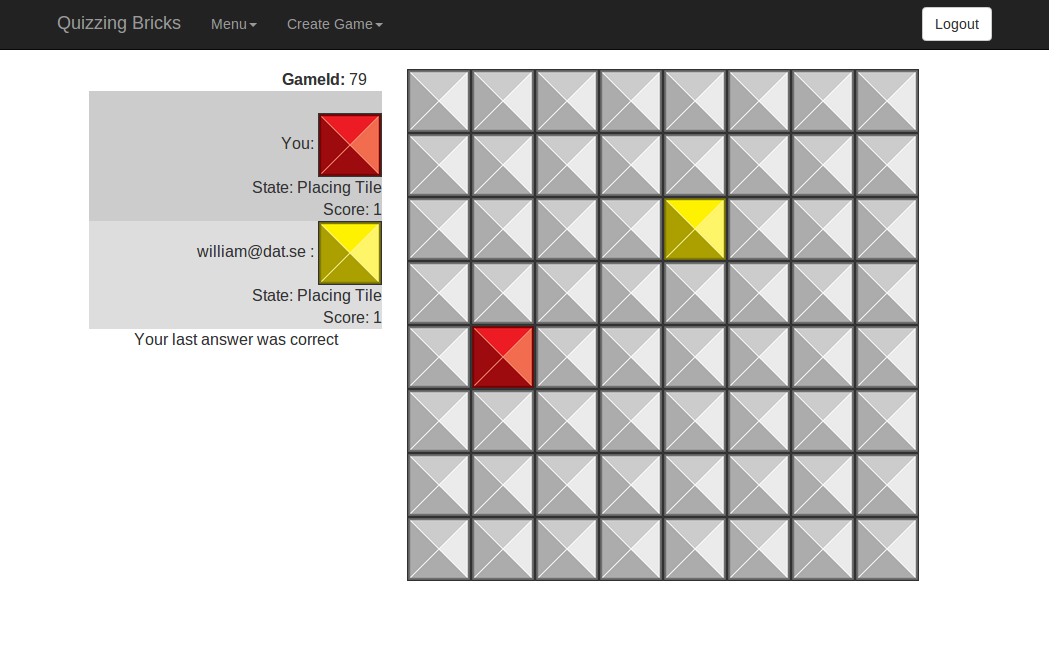
\includegraphics[width=\textwidth,height=\textheight,keepaspectratio=true]{img/game_board_page.png}
	\caption{The client website during a game.}
	\label{fig:web}
\end{figure}

As shown in Figure \ref{fig:web} the game board page basically contains a player status container on the left giving information about the color of the different players and their current game status (if they're placing tiles / answering question etc) and their current score in the game. On the Right side there's  a game board which is build with a grey base tile which is overwritten by the corresponding players tile when they have won that specific tile, this game board is of the size 8x8 in the current version but can easily be expanded by changing the loop variable for creating the board.

\subsection{Mobile Clients}
One focus in the design was that the applications should look and handle the same way. This was later determined to not be the best approach because of the differences between android and iOS design guidelines. The functionality in Android and iOS handles the same with some minor differences concerning the placement of where you can find and handle lobbies.\\
The only other major difference is, as mentioned before, the graphic design and what additional libraries we use for example communication. 



	\section{Technologies}
	The project is built with several technologies with key components built with the programming languages Python and Scala with support of different libraries and toolkits.

\subsection{Tools}
\subsubsection{Git}
The version control system used in the project was Git\cite{ref_git} and hosted on \url{http://github.com} because we all had some previous experience with this setup. On github we used a shared organization account (\url{http://github.com/quizzingbricks}) with our repositories and let the contributors to fork the main repository and send pull requests to merge back into the main repository.
\subsubsection{Vagrant}
Vagrant\cite{ref_vagrant} is a tool that lets developers create and use reproducible and portable environments. We chose to use Vagrant because we wanted all developers to share a common view with all tools pre-installed and let each developer focus on coding rather than operations and configure its own machine. The same provisioning script to install all packages in the virtual machine was also used on the server in our production environment with some additional configuration. 
\subsubsection{OpenStack}
OpenStack\cite{ref_openstack} is an open source platform for private and public clouds similar to Amazon's Web Services (AWS) and Google's Cloud Platform. Since we used Vagrant for our local development environment the task to deploy and manage the staging and production environment for the virtual machines was easy because the same provision of installable packages was re-used in the OpenStack as well which enabled us to have the same environment in development and production.

\subsection{Backend}
\subsubsection{Python and Gevent}
The Python language\cite{ref_python} is a general-purpose and high-level dynamic programming language and is used for most of our internal services (read more below about services in section \ref{zmq_protobuf}) and the web client and also our HTTP-based RESTful API that power our mobile clients. Gevent\cite{ref_gevent} is a coroutine-based networking library that enable event-driven concurrency in Python instead of thread-based concurrency. The use of gevent and non-blocking I/O enable the services and HTTP-based web and RESTful API to allow higher concurrency and more simultaneous connections which is used for websockets that the API and web client expose.
\subsubsection{Scala and akka}
Scala\cite{ref_scala} is a programming language which is syntactically close to its ancestor Java and can also be compiled to Java bytecode and use Java libraries directly in its code. The powerful object-oriented concepts in Java are included in Scala, but Scala also features extensive capabilities for functional programming, which include many features found in many purely functional languages such as pattern matching, immutability and lazy evaluation. Scala also extends the type system of Java into a unified type system together with higher-order types including co- and contravariant structures. It supports immutability and provides language and library means for writing code completely free of side-effects if desired.\\
Included in the native library of Scala is akka\cite{ref_akka}, which is a toolkit written for the Java platform that provides a framework for writing concurrency-based code through an implementation of the actor model of synchronous computing. Actors are objects that are constructed in a hierarchical fashion to allow for supervision and failover and communicate through a message mechanism. The akka toolkit is intended to provide for scalability by allowing each actor to seamlessly serve as an abstraction for anything from a thread to a server cluster.
\subsubsection{$\varnothing$MQ and Protocol Buffers\label{zmq_protobuf}}
$\varnothing$MQ\cite{ref_zmq} is a socket library that enhances the socket programming and includes multiple message patterns were we use request/reply and publish/subscribe. Request/reply is used for client/server communication and publish/subscribe is used as a single publisher publish messages to potentially multiple listeners. Google's Protocol Buffers\cite{ref_protobuf} is a serialization format that enables multiple languages to share the same transport format and protocol. Another popular method is to use a RESTful API over HTTP with JSON as transport format. As we evaluated the combinations we ended up with the ZeroMQ and Protocol Buffer approach since the HTTP adds an overhead on the TCP and also because we designed the protocol to only use request/reply without any special features that HTTP enables but also since we needed publish/subscribe and that is not supported by HTTP.
\subsubsection{Database Technologies}
For persistence of data, the relational database system PostgreSQL\cite{ref_postgres} is used, which is accessed through the SQLAlchemy\cite{ref_sqlalchemy} toolkit for the Python language, and the Slick\cite{ref_slick} toolkit for Scala. The tool Alembic\cite{ref_alembic} has been used to migrate between database versions during development.

\subsection{iOS 7}
The iOS client needs to be written in Objective C and the only choice you have is trying to use a third party development tool that translates code into objective c. The problem with these tools is that they actually restrict you even further than Apple does with their tools and you end up with an application that doesn't feel good enough, so we decided to develop directly in Xcode using objective c. Apple provides a foundation framework that actually includes all the things we needed for our application from Strings to url requests and json parsing so no use for external libraries has arisen. 

\subsection{Android}
Android uses java and xml to make applications, the graphical design is most often done in xml and uses java for functionality. But the graphic can be made in java as well, which allows for dynamic layouts compared to xml's static layouts. 
This project focused on developing for Android phones running version 4.0 (Ice Cream Sandwich) and above. The main reason for this decision is that the percentage of devices running older version is around 20\%\cite{ref_android_versions} and by excluding the backwards compatibility more focus could be put on making a better ui using the newer API:s. This also gives our application more of a modern look which is harder to mimic with the older API versions.
As for the development environment there are two official choices offered by Google, Android Studio and Eclipse. For this project we choose to work with Eclipse since Android Studio is still in beta. But as a IDE Eclipse has some flaws and one of the major ones is the amount of files that are included in each project which makes backing up files an unnecessary hassle.

\subsection{Web}
\subsubsection{HTML5}
HTML Is a markup language used for structuring and presenting information on the Internet. HTML5\cite{ref_html5_1}\cite{ref_html5_2} is the latest iteration of the HTML standard. And is more closely working with JavaScript (JS) and Cascading Style Sheets (CSS). This technology has mainly been used for the above reason that is structuring and presenting the information on our web platform. Where Bootstrap has been the backbone in the design with the navigation bar layout and grid layouts for the body of the webpage and basic clean CSS. In addition to this JS has been used for additional functionality on the game board page. 
\subsubsection{Websockets}
Websockets\cite{ref_websocket} is a protocol that got full-duplex communication channel of a single TCP connection. In the web applications it have been used to receive message containing information about changes of the game and player states in the backend. When these messages was received they called JS functions that updated the game board as soon as a full game round have been completed, they are also used to change the player status for a specific player whose state was changed.
\subsubsection{Flask}
Flask\cite{ref_flask} is a micro framework written in Python and is based on Werkzeug WSGI toolkit and the template engine Jinja2\cite{ref_jinja2}. Flask is used to implement the HTTP end-points for both the web application and the RESTful API that is used by the mobile clients.



	\section{System Architecture}
	\begin{figure}[H]
	\centering
	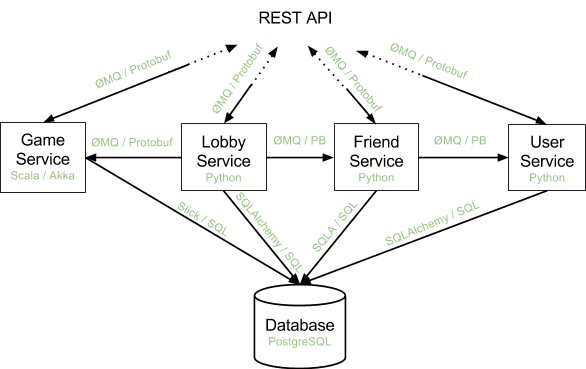
\includegraphics[width=\textwidth,height=\textheight,keepaspectratio=true]{img/sPVjzeXSLniaBJWqfNTsV4A.png}
	\caption{The infrastructure of the server backend. Each arrow indicates communication between respective services and green text indicates the main technologies used for the various entities.}
	\label{fig:sysarch}
\end{figure}

\subsection{Backend}
The backend is divided into smaller parts and composed as services that run as independent processes, where each service handles a distinct part of the business logic. To enable services to talk between each other ZeroMQ is used as the transport layer and Protocol Buffers is employed as the serialization or transport format to enable different languages to share the same protocol. ZeroMQ readily allows for implementation of message patterns such as the request/reply model and the publish/subscribe paradigm, and we have used the former pattern for the primary communication between processes and the latter pattern for websocket push notifications.
An easily extendable architecture for the Python processes is built based on an inheritable base class that together with a shared protocol structure allows for quick development of new services. The architecture also allows for expedient definition of new methods that are callable by RPC messaging via ZeroMQ and Protocol Buffers. 

\subsubsection{Game Service}
Built with scalability in mind, the game process handles all the game logic in individual games, as well as the creation and maintenance of new games, and the pruning of old games. Internally, the game utilizes a load broker pattern for load balancing to allow many ZeroMQ requests to be handled simultaneously, and uses Akka to parallelize the requests. The Slick API is used throughout to save game state to the database.

\subsubsection{Lobby Service}
This is a service that handles the creation of games. This service has functionality to create a lobby, remove a lobby and start a game. When a user has created a lobby the user can send invitations to friends and the friends can accept or deny these invitations. This service is used when a user checks which lobbies said user is a member of. 

\subsubsection{User Service}
This service handles the users of the system. The service has functionality to authenticate, create and get users. The service is used when a user is created and when a user logs in. When a user tries to add another user as a friend this service is used to make sure that the provided email address for the friend really exists. 

\subsubsection{Friends Service}
This is a service that handles the users connection with friends. The service gives the functionality to add a friend, remove a friend or to list all friends. The service is used when a user manages the friends list. It is also used while creating a game. The user can choose friends from the current friends list whom the user wishes to play with and invite them to a game lobby.

\subsection{Web/RESTful API}
As can be seen in Figure \ref{fig:sysarch} the REST API is in the top and can call the different services with protocol buffers messages over ZMQ. The Web application Flask server is just like the REST API located in the top and use the services in the same manner as the REST API.

\subsection{Mobile Clients}
The mobile clients communicate with the backend using the web api, this communication is made using simple http-requests to different urls with custom headers such as user-token and sometimes providing data using a body of json. The responses are either just a verification that the request was made successfully or a body of json with information. Creating and handling these requests and responses in each and every view directly would be tedious and unnecessary so the focus and most work for each client has been creating a communication manager that handles these requests as easily as possible. We wanted these communication managers to be made in such a way that you could easily expand upon them when new features are added to the backend. The android and iOS client has each achieved this in a different way but achieved it nonetheless. 

\subsection{Security}
The security for the systems can be seen as two different parts. The first one is the security for the RESTful API that mobile clients consume and produce data to and the other is the web frontend. Both the RESTful API and the web frontend share the same backend and the libraries used in the backend to access the database, SQLAlchemy and Slick automatically protect against SQL Injections if used in the recommended way which is done against both libraries.

\subsubsection{RESTful API}
Today the most popular security scheme used by platforms and applications is the OAuth 2.0\footnote{http://oauth.net/2/} which is used by the larger actors to provide public available API's, such as Facebook, Google or Github. The main difference related to our project is that we don't expose a public API in that sense, since we don't plan to allow 3rd party developers to create their own clients. Because our API is private, our authentication scheme is more simple than the fit-for-all OAuth 2.0 scheme. 

The security scheme for our mobile clients is that the user provide the email and password in the mobile client and transmit the data over the network to the RESTful API to exchange the email/password-credentials for an access token. The access token is then used instead of the email and password during requests to the RESTful API by the mobile client when it needs to acts on behalf for the user. 

The access token is a signed token that contains the user id for the authenticated user and a timestamp when the token were obtained which means that the end-user can read the values from the token, but not change it due the signature unless the end-user in some way have got access to the secret key that is kept on the server. To limit the eventual spread of access tokens, they are only valid during a limited period and in our case it is 7 days and after that the user is required to request a new token by the email and password credentials. During development and the demos running on the production server, all communication have been done without TLS, but in a real scenario TLS is of course required to protect the users data that is transmitted over the wire.
\subsubsection{Web frontend}
The authentication scheme on the frontend is based on session cookies which means that the user provides email and password and is then logged in by storing a signed cookie, similar to the approach described in the RESTful API security, but simpler and without the timestamp. The web frontend is protected to the most common security vulnerability Cross-Site Scripting\footnote{https://www.owasp.org/index.php/XSS} (XSS) since the templating system provided by Flask (Jinja2) by default escapes the output and no known security vulnerabilities exist as today in Jinja2 that enables XSS. Other common vulnerabilities such as Cross-Site Request Forgery\footnote{https://www.owasp.org/index.php/CSRF} (CSRF) is not secured by default and such attacks are possible to do as today, like add or remove friends and possibility to fetch or answer a quiz question.


	\section{Result}
	\subsection{User Experience}
\subsubsection{Login / Register}
For the login we choose to use the email as the users unique identifier and a password for the means of authentication. The main reason for going with a username and password authentication instead of a oauth solution is because this solution can be used without having a third party account. Implementing an oauth solution that everyone can use is time consuming because you would need to have more than one implementation (like Google+, Facebook or Twitter login methods) and therefore not fitting for the time scope of the project. This means that a username and password system would need to be implemented in case a user has no accounts on the given services. The main drawback with this kind of login method is that it requires the user to remember a new password instead of using an already existing username and passphrase. 
\subsubsection{Friends Management}
To make the process of inviting friends to the game more easy we choose to implement a friends list feature.\\ 
Friends are added to the friends list by entering their email address and after that they can be invited to any lobby by just a single click or tap. Our implementation does not require the other party to accept the friends request (like in a social network) and the major reason for that is because our friends list is more suppose to behave like a shortcut for inviting friends to the game. Having the other party accepting a friends request is therefore unnecessary since our application doesn't limit how users can send invitations to each other. This is however a feature that needs to be considered if the number of social features increase in the application (like a chat feature for instance).
\subsubsection{Lobby}
The lobby was chosen to allow users to make a party of friends before going into a game. 
\bigskip
The owner of a lobby may choose to invite how many friends he/she wishes for, however there are only 2 or 4 slots that may be filled (the owner takes one slot), how many slots there are depends on the game type. The remaining users may not join the lobby when it has become full. The owner may however start the game at any time, in such an occasion the lobby will become locked from joining by invitation.\\ 
The lobby will then be placed in a queue depending on game type and how many players are currently in the game. The lobby then becomes merged with other lobbies until such a time that all slots are filled, the lobby will then be sent to the game service to become a game.
\subsubsection{Game}
When a game starts it will be added to the games list where it can have two different kinds of states, waiting for other players and ready to place brick.\\
The game board itself is represented by bricks which is placed in an eight by eight square. White bricks are untaken places on the board and the players bricks are represented in different colors. The board view also includes a list showing which colors the players have.\\
When a user wants to place a brick on the board he/she first picks a position on the board, if it's a legal move the user will be prompted with a question. In this state the user can either answer correctly or incorrectly to the question and also time out if a answer has not been given after 20 seconds. When a question times out it will act as a false answer. If more than one player has chosen the same brick and answered correctly to the question there will be a "Question Battle" to determine which player gets the brick. In a question battle the players will each get a new question, if a player answers incorrectly to a question they are out. If more than one player answers correctly to a question they will all be given a new question. The question battle continues until there are either one player or no one left. In the case of the second outcome (where all of the users has answered incorrectly to the current question) no one will receive the brick and it will be left untaken in the second round.\\
If a player has answered the question correctly the brick on the chosen position will either get their color or a lighter version of it. The second option acts as a placeholder when there still are players in the game that haven't picked a place to place their bricks. This is to to give a visualisation to the placing of the brick and to inform the player that it might be a question battle over it.\\ 
When all the players have placed their bricks and all the question battles are over a new round will begin.
\subsubsection{Cross Platform}
The application created for this project is available on a total of three platforms and a user can switch between them. All of the platforms have the same features so you don't lose any part of the core experience when on one of the applications. The big difference between all of the clients is that they have different user interfaces as we chose to follow the platform guidelines for user interfaces.\\
Because the state of the game is controlled by the server it means that a user can log in to any of the three devices and resume their game where they left of. This gives the users more freedom in how they chose to interact with the application, whether it being on a big screen pc or a portable device on the go. It also means that a user can, for instance, start a new game on the web browser at home and play the next round on the daily commute on the bus.

\subsection{Project Goals}
\subsubsection{Scalability}
Through the use of APIs such as Gevent and Akka, we have provided a scalable sub-architecture inside each process that allows the backend to efficiently utilize available computing resources to serve a very large number of clients simultaneously. Therefore, we feel that we have achieved our initial goal to provide the necessary level of scalability for a project of this character.
\subsubsection{Extensibility}
Since we have purposely divided the backend into subcomponents implemented as processes and have provided an infrastructure that is constructed with extensibility in mind, we have provided ample and powerful means to readily expand the backend with new processes and modules. We deem that we have satisfied our objective of being able to easily extend the system with new functionality.
	
	\section{Discussion}
	\subsection{Development Issues}
When we planned the project we decided that with so many members we could create both an Android and an iOS client to prove how cross platforming would work. This meant setting two people to work on the android client and one on the iOS client thinking that the clients would be done in good time before the end of the course. Unfortunately we did not consider the steep learning curve of creating a full application with little previous experience. This meant that the three people set to work on the clients were pretty much locked in to clients with too much work spent to scrap them when we realised that they would take the full extent of the course to complete. So in hindsight we would probably have gone with only one of the mobile clients. 

Another problem we had was the difficulty in getting something to work as early as possible without being completely done with it. Most features we implemented were unusable until they were finished since we set to make them as good as we wanted them to be for the finished product from the beginning. This is probably where most of us have learned most from our mistake since it is so much more useful to have a bare bone working prototype to share with the team than nothing at all until you have a finished product. Especially since you are unlikely to have achieved a finished product without testing it with the team. 

In both the android and the iOS client the focus has been to get all features working and not in trying to make a beautiful designed interface shared between devices. So for each client we've stuck to the standard way of making a simple application. This has lead to some minor differences between the mobile clients but we believe that trying to for example recreate the iOS layout in the android phone or vice versa would only confuse the user more since an android or iOS user expects an application to work in a certain way when using an android or iOS device. 
\subsection{Future Work}
The most prominent work would be to actually launch the application. What is stopping us today is that we have no questions for our quiz game, for this purpose we would need to buy a service providing this.
For the application designs on web and the mobile clients more time could be spent on graphical design to make the clients look better, also reducing the clicks needed to do things inside the application by using  ``smart'' patterns or additional settings so you for example, automatically accept invite from a player etc.
For the game itself, one can think of developing additional game modes that you can choose to play.

	
	\section{Conclusion}
	\input{7conclusion}
	
	%refs
	\bibliographystyle{unsrt}
%include bibliography file 9ref.bib
\bibliography{9ref}

	
	\newpage
	\appendix
	\section{API}
	The API\cite{ref_api} is segmented into four different parts each describing the main responsibility of that section.

\subsection{Users}

\subsubsection{/api/users/}        
\tab   	Sent\\
\tab\tab	\textbf{Post} email="email@example.com", password="password"\\
\tab   	Response\\
\tab\tab 	200 ok\\
\tab   	Response fail\\
\tab\tab   	\{"errors":\{"message":"Internal service error", "code": "000"\}\}\\
\tab\tab   	\{"errors":\{"message":"This mail is already taken","code":"101"\}\}\\
\tab\tab   	\{"errors":\{"message":"Missing email or password","code":"102"\}\}\\
\tab\tab	\{"errors":\{"message":"Service not available", "500"\}\}\\
\tab\tab	\{"errors":\{"message":"Error code not defined","code:"0"\}\}\\

\subsubsection{/api/users/login/}
\tab    Sent\\
\tab\tab	\textbf{Post} email="email@example.com", password="password"\\
\tab	Response\\
\tab\tab	\{"token":"abcdefghijklmnopqrstuvwxyz1234567890"\}\\
\tab	Response fail\\
\tab\tab	\{"errors":\{"message":"Wrong email or password","code":"010"\}\}\\
\tab\tab	\{"errors":\{"message":"Internal service error","code":"000"\}\}\\
\tab\tab	\{"errors":\{"message":"E-mail or password is missing, check your data", "1"\}\}\\
\tab\tab	\{"errors":\{"message":"Service not available", "500"\}\}\\
\tab\tab	\{"errors":\{"message":"Error code not defined","code:"0"\}\}\\

\subsubsection{/api/users/me/}
\tab	Sent\\
\tab\tab	\textbf{Get} token="$<$tok\_id$>$"\\
\tab	Response\\
\tab\tab	\{"id":"$<$u\_id$>$", "email":"$<$mail\_address$>$"\}\\
\tab	Response fail\\
\tab\tab	\{"errors":\{"message":"The token is invalid, please login again","code":"1"\}\\

\subsection{Friends}

\subsubsection{/api/users/me/friends/}
\tab	Sent\\
\tab\tab	\textbf{Get} token="$<$tok\_id$>$"\\
\tab\tab	\textbf{Post} token="$<$tok\_id$>$", friend = "$<$email$>$"\\
\tab	Response\\
\tab\tab	\textbf{Get:}\tab	\{friends : $[$\{"id":"$<$u\_id1$>$","email":"$<$mail\_address$>$"\},..$]$\}\\
\tab\tab	\textbf{Post:}\tab	Plaintext "OK"\\
\tab	Response fail\\
\tab\tab	\{"errors":\{"message":"Missing required friend parameter", "004"\}\}\\
\tab\tab	\{"errors":\{"message":"no such user exists","code:"0"\}\}\\
\tab\tab	\{"errors":\{"message":"The token is invalid, please login again","code":"100"\}\}\\
\tab\tab	\{"errors":\{"message":"Service not available", "500"\}\}\\
\tab\tab	\{"errors":\{"message":"Internal service error", "000"\}\}\\

\subsubsection{/api/users/me/friends/$<$user\_id$>$/}
\tab	Sent\\
\tab\tab	\textbf{Delete} token="$<$tok\_id$>$"\\
\tab	Response\\
\tab\tab	Plaintext "OK"\\
\tab	Response fail:\\
\tab\tab	\{"errors":\{"message":"no such user exists","code":"011"\}\\
\tab\tab	\{"errors":\{"message":"The token is invalid, please login again","code":"100"\}\\
\tab\tab	\{"errors":\{"message":"Service not available", "500"\}\}\\
\tab\tab	\{"errors":\{"message":"Internal service error", "500"\}\}\\


\subsection{Lobby}
\subsubsection{/api/games/lobby/}
\tab	Sent\\
\tab\tab	 \textbf{Get} token="$<$tok\_id$>$"\\
\tab	Response\\
\tab\tab	\{"lobbies": $[$\\
\tab\tab\tab	\{\\
\tab\tab\tab	"l\_id": $<$l\_id$>$, \\
\tab\tab\tab	"owner" : $<$bool$>$, \\
\tab\tab\tab	"size": $<$size\_int$>$, \\
\tab\tab\tab	"invited\_count":$<$int$>$, \\
\tab\tab\tab	"accepted\_count" : $<$int$>$\\
\tab\tab\tab	\}, ...\\
\tab\tab	$]$\}\\
\tab	Response fail\\
\tab\tab	\{"errors":\{"message":"The token is invalid, please login again","code":"100"\}\\
\tab\tab	\{"errors":\{"message":"Service not available","code":"500"\}\}\\
\tab\tab	\{"errors":\{"message":"Internal service error","code":"500"\}\}\\

\subsubsection{/api/games/lobby/}
\tab	Sent\\
\tab\tab	\textbf{Post} token="$<$tok\_id$>$" size="$<$size$>$"\\
\tab	Response\\
\tab\tab	\{"lobby": \{\\
\tab\tab\tab	"l\_id" : $<$l\_id$>$,\\
\tab\tab\tab	"size" : $<$int$>$,\\
\tab\tab\tab	"owner" : $<$bool$>$,\\
\tab\tab\tab	"players" : $[$\{\\
\tab\tab\tab\tab	"u\_id" : $<$u\_id$>$,\\
\tab\tab\tab\tab	"u\_mail" : $<$string$>$,\\
\tab\tab\tab\tab	"status" : "accepted"/"waiting"\\
\tab\tab\tab\tab	\},...$]$\\
\tab\tab\tab	\}\\
\tab\tab	\}\\
\tab    Response fail\\
\tab\tab	\{"errors":\{"message":"The token is invalid, please login again","code":"100"\}\\
\tab\tab	\{"errors":\{"message":"Missing required parameter size","code":"004"\}\}\\
\tab\tab	\{"errors":\{"message":"Service not available","code":"500"\}\}\\
\tab\tab	\{"errors":\{"message":"Internal service error","code":"400"\}\}\\
\tab\tab	\{"errors":\{"message":"Internal server error","code":"500"\}\}\\

\subsubsection{/api/games/lobby/$<$l\_id$>$/}
\tab	Sent \\
\tab\tab	\textbf{Get} token="$<$tok\_id$>$"\\
\tab	Response \\
\tab\tab	\{"lobby":\\
\tab\tab\tab	\{"l\_id"="$<$l\_id$>$", \\
\tab\tab\tab	"size":$<$size\_int$>$, \\
\tab\tab\tab	"owner":True/False, \\
\tab\tab\tab	"invited\_count": $<$int$>$,\\
\tab\tab\tab	"accepted\_count": $<$int$>$, \\
\tab\tab\tab	"players\footnote{Should be sorted as Owner$>$Accepted$>$Waiting}" : $[$\{\\
\tab\tab\tab\tab	"u\_id" : $<$u\_id$>$, \\
\tab\tab\tab\tab	"u\_mail" : $<$string$>$,\\
\tab\tab\tab\tab	"status": "accepted"/"waiting"\},...\\
\tab\tab\tab\tab	$]$\}\\
\tab\tab	\}\\
\tab	Response fail\\
\tab\tab	\{"errors":\{"message":"The token is invalid, please login again","code":"100"\}\\
\tab\tab	\{"errors":\{"message":"Lobby does not exist","code":"226"\}\\
\tab\tab	\{"errors":\{"message":"You are not permitted to that lobby","code":"42"\}\\
\tab\tab	\{"errors":\{"message":"Internal service error","code":"400"\}\}\\
\tab\tab	\{"errors":\{"message":"Service is not available","code":"500"\}\}    \\

\subsubsection{/api/games/lobby/$<$l\_id$>$/accept/}
\tab	Sent\\
\tab\tab	\textbf{POST} token="$<$tok\_id$>$"\\
\tab	Response\\
\tab\tab	Plaintext "OK"\\
\tab	Response fail\\
\tab\tab	\{"errors":\{"message":"There exists no such lobby","code":"226"\}\}\\
\tab\tab	\{"errors":\{"message":"You are not permitted to that lobby","code":"42"\}\}\\
\tab\tab	\{"errors":\{"message":"The lobby is full","code":"225"\}\}\\
\tab\tab	\{"errors":\{"message":"Service not available","code":"500"\}\}\\



\subsubsection{/api/games/lobby/$<$l\_id$>$/deny/}
\tab	Sent\\
\tab\tab	\textbf{Post} token="$<$tok\_id$>$"\\
\tab	Response\\
\tab\tab	Plaintext "OK"\\
\tab	Response fail\\
\tab\tab	\{"errors":\{"message":"The token is invalid, please login again","code":"100"\}\}\\
\tab\tab	\{"errors":\{"message":"The lobby is full","code":"225"\}\}\\
\tab\tab	\{"errors":\{"message":"There exists no such lobby","code":"226"\}\}\\
\tab\tab	\{"errors":\{"message":"You are not permitted to that lobby","code":"227"\}\}\\
\tab\tab	\{"errors":\{"message":"Service not available","code":"500"\}\}\\

\subsubsection{/api/games/lobby/$<$l\_id$>$/invite/}
\tab	Sent \\
\tab\tab	\textbf{Post\footnote{Header should be \tt{Content-Type = "application/json"}}} token="$<$tok\_id$>$", invite = \{ "invite" : $[$$<$u\_id1$>$, $<$u\_id2$>$, ...$]$\}\\
\tab	Response\\
\tab\tab	Plaintext "OK"\\
\tab	Response fail\\
\tab\tab	\{"errors":\{"message":"Required JSON body is missing or bad type, check your content-type","code:"0"\}\}\\
\tab\tab	\{"errors":\{"message":"Required JSON body is missing or bad type","code":"004"\}\}\\
\tab\tab	\{"errors":\{"message":"The token is invalid, please login again","code":"100"\}\\
\tab\tab	\{"errors":\{"message":"There exists no such lobby", "code": 226\}\}\\
\tab\tab	\{"errors":\{"message":"You are not permitted to that lobby","code":"42"\}\\
\tab\tab	\{"errors":\{"JSON object invite should be an array with only integers","code":"004"\}\}\\
\tab\tab	\{"errors":\{"message":"Service not available","code":"500"\}\}\\
\tab\tab	\{"errors":\{"message":"Internal service error","code":"0"\}\}\\


\subsubsection{/api/games/lobby/$<$l\_id$>$/start/}
\tab	Sent\\
\tab\tab	\textbf{Post} token="$<$tok\_id$>$"\\
\tab	Response\\
\tab\tab	Plaintext "OK"\\
\tab	Response fail\\
\tab\tab	\{"errors":\{"message":"The token is invalid, please login again","code":"100"\}\\
\tab\tab	\{"errors":\{"message":"There exists no such lobby","code":"226"\}\\
\tab\tab	\{"errors":\{"message":"You are not permitted to that lobby","code":"42"\}\\
\tab\tab	\{"errors":\{"message":"Service not available","code":"500"\}\}   \\ 

\subsubsection{/api/games/lobby/$<$l\_id$>$/end}
\tab	Sent\\
\tab\tab	\textbf{Post} token="$<$tok\_id$>$"\\
\tab	Response\\
\tab\tab	Plaintext "OK"\\
\tab	Response fail\\
\tab\tab	\{"errors":\{"message":"The token is invalid, please login again","code":"100"\}\\
\tab\tab	\{"errors":\{"message":"You are not permitted to that lobby","code":"42"\}\\
\tab\tab	\{"errors":\{"message":"Service not available","code":"500"\}\}\\


\subsection{Games}
\subsubsection{/api/games/}
\tab	Sent\\
\tab\tab	\textbf{Get} token=$<$"tok\_id"$>$\\
\tab	Response\\
\tab\tab	\{"games":$[$\{"id": $<$int$>$, "size": $<$int$>$, "state": $<$int$>$\}, ...$]$\}\\
\tab	Response fail\\
\tab\tab	\{"errors":\{"message":"The token is invalid, please login again","code":"100"\}\\
\tab\tab	\{"errors":\{"message":"Service is not available","code":"500"\}\}\\

\subsubsection{/api/games/$<$g\_id$>$/\label{statehere}}
\tab	Sent\\
\tab\tab	\textbf{Get} token=$<$"tok\_id"$>$\\
\tab	Response\\
\tab\tab	\{"gameId" : $<$int$>$, \\
\tab\tab	"players": $[$     \{     \\
\tab\tab\tab	"userId" : $<$int$>$,\\
\tab\tab\tab	"email" : $<$string$>$,\\
\tab\tab\tab	"state\footnote{0 can place\\\tab1 can get question\\\tab2 is answering\\\tab3 waiting\\\tab4 Lost\\\tab5 Won}" : $<$int$>$,\\
\tab\tab\tab	"x" : $<$int$>$,\\
\tab\tab\tab	"y" : $<$int$>$,\\
\tab\tab\tab	"score" : $<$int$>$,\\
\tab\tab\tab	"answeredCorrectly" : $<$bool$>$\\
\tab\tab\tab	\}, \{...\},...\\
\tab\tab	$]$,\\
\tab\tab	"board" : $[$$<$int$>$, ..$]$\}\\
\tab	Response fail\\
\tab\tab	\{"errors":\{"message":"Game service not available","code":"500"\}\}\\


\subsubsection{/api/games/$<$g\_id$>$/play/move}
\tab	Sent\\
\tab\tab	\textbf{Post} token="$<$tok\_id$>$", x="$<$x\_coord$>$", y="$<$y\_coord$>$"\\
\tab	Response \\
\tab\tab	200 ok\\
\tab	Response fail\\
\tab\tab	\{"errors":\{"message":"Some of the required parameters x and y are missing","code":"004"\}\\
\tab\tab	\{"errors":\{"message":"Service not available","code":"500"\}\}\\
\tab\tab	\{"errors":\{"message":"Game service not available","code":"500"\}\}\\
\tab\tab	\{"errors":\{"message":"The token is invalid, please login again","code":"100"\}\\

\subsubsection{/api/games/$<$g\_id$>$/play/question}
\tab	Sent\\
\tab\tab	\textbf{Post} token="$<$tok\_id$>$"\\
\tab	Response\\
\tab\tab	\{"question":"$<$String$>$" "alternatives":$[$"$<$a1$>$","$<$a2$>$",..$]$ \}\\
\tab	Response fail\\
\tab\tab	\{"errors":\{"message":"Service not available","code":"500"\}\}\\
\tab\tab	\{"errors":\{"message":"Game service not available","code":"500"\}\}\\

\subsubsection{/api/games/$<$g\_id$>$/play/answer}
\tab	Sent\\
\tab\tab	\textbf{Post} token="$<$tok\_id$>$", answer="$<$Int$>$" \\
\tab	Response\\
\tab\tab	\{ "isCorrect" : $<$bool$>$ \}\\
\tab	Response fail\\
\tab\tab	\{"errors":\{"message":"Missing required parameter answer","code":"400"\}\\
\tab\tab	\{"errors":\{"message":"The token is invalid, please login again","code":"100"\}\\
\tab\tab	\{"errors":\{"message":"Service not available","code":"500"\}\}\\
\tab\tab	\{"errors":\{"message":"Game service not available","code":"500"\}\}\\


\subsubsection{/api/games/$<$g\_id$>$/events} 
\tab	Sent\\
\tab\tab	\textbf{Post} token="$<$tok\_id$>$", answer="$<$Int$>$" \\
\tab	Response\\
\tab\tab	\{     "type" : "player\_change" , \\
\tab\tab	"payload": \{ \\
\tab\tab\tab	"player": \{\\
\tab\tab\tab\tab	"id" : $<$u\_id$>$, \\
\tab\tab\tab\tab	"state\footnote{see section \ref{statehere}}": $<$s$>$,\\
\tab\tab\tab\tab	"score": $<$int$>$\\ 
\tab\tab\tab\tab	\}\\
\tab\tab\tab	\}\\
\tab\tab	\}\\
    
\tab\tab	or\\

\tab\tab	\{    "type": "board\_change",\\
\tab\tab	"payload": \{\\
\tab\tab\tab	"board": $[$$<$b1$>$,..$]$,\\
\tab\tab\tab	"players": $[$\{\\
\tab\tab\tab\tab	"id" : $<$u\_id$>$, \\
\tab\tab\tab\tab	"state" : $<$s$>$, \\
\tab\tab\tab\tab	"score": $<$int$>$\\
\tab\tab\tab	\}, \{...\}, ...$]$\\
\tab\tab	\}\\
\tab	Response fail\\
\tab\tab	\{"type":"unknown","payload":\{"msg\_type":$<$msg\_type$>$\}\}\\
\tab\tab	\{"type":"type","player\_change":\{"payload":\{"player":\\
\tab\tab\tab	\{"id":$<$id$>$,"state":$<$state$>$,"score":$<$int$>$\}\}\}\\

	
	\newpage
	\appendix
	\section{Game Rules}
	A game allows for either two or four players and consists of a series of turns, where at the start of each turn, each player decides where to place a brick on a game board of size 8x8. 
After each player has chosen where to put their brick, the player is able to request a question. After having received the question, they have to answer it correctly within a small amount of time to be allowed to place their brick on the chosen position. After this, a new turn starts. If two or more players have chosen the same position, each of those players will be asked more questions until no more than one person has answered correctly to all of the questions. When a player gets his brick added to the board, he gets a number of points added to his score that is equal to the total number of contiguous bricks that can be traced through the newly acquired position, in a linear fashion, horizontally, vertically and diagonally. The player with the highest score when the score count of any player has reached 50 has won the game.


\end{document}